
% These macros come from my dissertation.
\newcommand{\cedge}[1]{\stackrel{#1}{\longleftarrow}}
\newcommand{\cred}[3]{\mathit{#1} \cedge{#3} \mathit{#2}}
\newcommand{\datalog}{\text{Datalog}}
\newcommand\T{\rule{0pt}{2.1ex}}

\startslide{Outline}
% The outline follows the structure of my dissertation. Why not?
\begin{cenumerate}
\item Introduction
\item Review of Trust Management
\item SpartanRPC/Sprocket
\item Scalaness/nesT
\item Evaluation
\item Conclusion
\end{cenumerate}
\stopslide

%%%%%

\startslide{Objective}
\centerline{\emph{\textbf{Trust Management Authorization in Sensor Networks}}}

\begin{citemize}
\item \cemph{Trust Management}: A way of authorizing access to resources in distributed, dynamic
  systems where principals don't know each other.

\item \cemph{Sensor Networks}: A kind of embedded system with limited CPU, memory, and available
  power.
\end{citemize}
\stopslide

%%%%%

\startslide{Two Solutions}
\begin{citemize}
\item \cemph{SpartanRPC}: An extension to the nesC programming language allowing secure RPC.

\item \cemph{Scalaness/nesT}: A staged programming system that allows an extended Scala to
  specialize and compose nesT modules.
\end{citemize}

\stopslide

%%%%%

\startslide{Language Based Approach}
Use programming languages to address the issues.

\begin{citemize}
\item \cemph{More efficient}: Compiler in a position to do optimizations.
\item \cemph{More robust}: Static analysis finds errors earlier.
\item \cemph{Easier to use}: Special syntax/semantics makes features more accessible.
\item \cemph{Better foundation}: Rigorous techniques, e.g. type theory, can guide design.
\end{citemize}
\stopslide

%%%%%

\startslide{SpartanRPC Motivation}
\centerline{\scalebox{1.0}{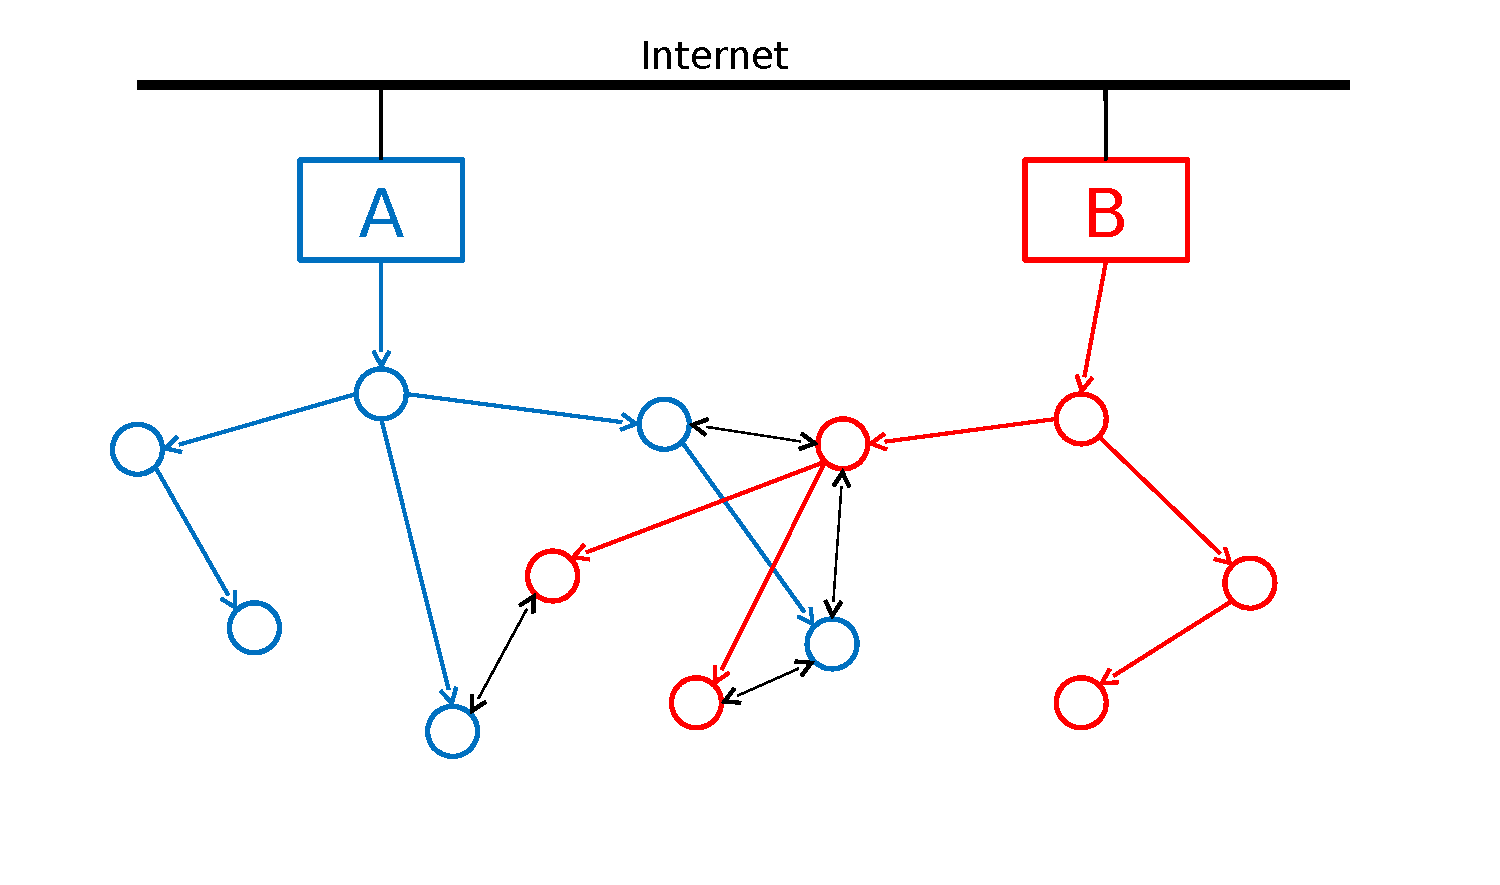
\includegraphics{Figures/SpartanRPC-Motivation.pdf}}}
\stopslide

%%%%%

\startslide{Scalaness Motivation}
\centerline{\scalebox{1.0}{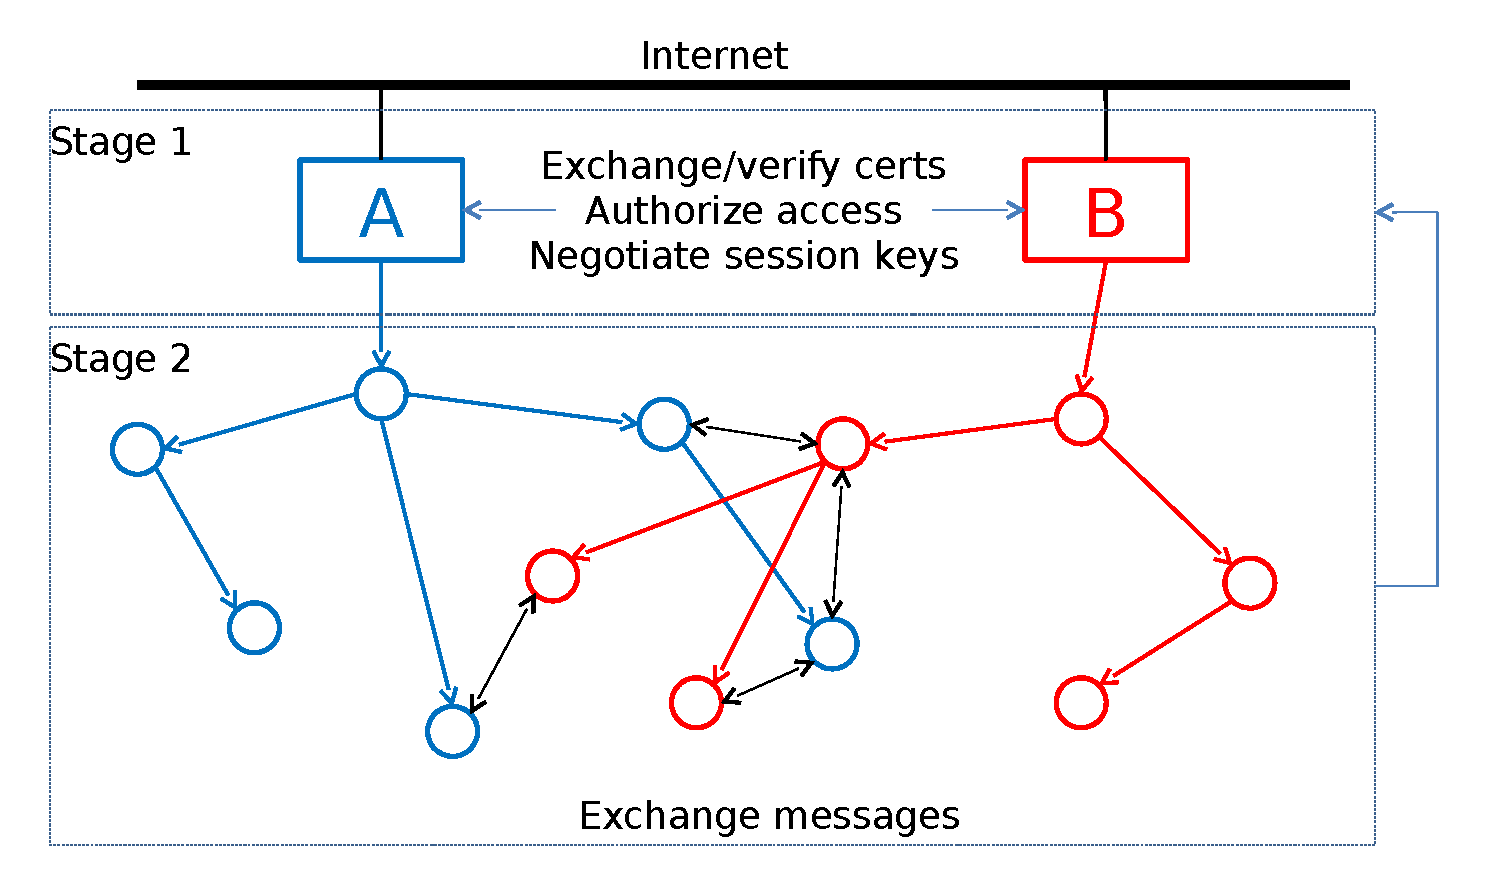
\includegraphics{Figures/Scalaness-Motivation.pdf}}}
\stopslide

%%%%%

\startslide{Application Possibilities}
\begin{citemize}
  \item Directed diffusion \& data aggregation
  \item In-network time synchronization
  \item Data collection (\cemph{Snowcloud})
  \item Mobile applications
  \begin{citemize}
    \item Querying infrastructure networks
    \item Body area networks
  \end{citemize}
\end{citemize}
\stopslide

%%%%%

\startslide{Outline}
\begin{cenumerate}
\item Introduction
\item \cemph{Review of Trust Management}
\item SpartanRPC/Sprocket
\item Scalaness/nesT
\item Evaluation
\item Conclusion
\end{cenumerate}
\stopslide

%%%%%

\startslide{Structure of Trust Management Systems}
\centerline{\scalebox{1.75}{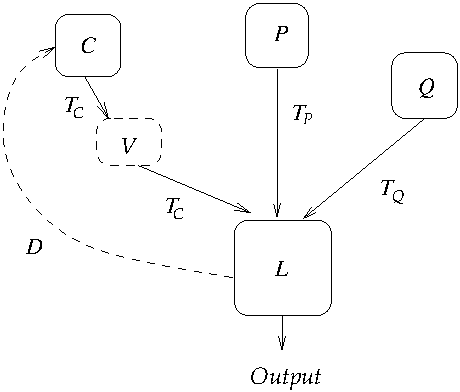
\includegraphics{Figures/tmstruct.pdf}}}
\stopslide

%%%%%

\startslide{$RT_0$ Credential Forms}
Simplest member of the $RT$ family\footnote{\textit{Design of a Role-based Trust-management
    Framework}; Li, Mitchell, Winsborough, 2002}.
\begin{cenumerate}
\item $\cred{A.r}{E}{}$ 
\item $\cred{A.r}{B.s}{}$ 
\item $\cred{A.r}{B.s.t}{}$ 
\item $\cred{A.r}{f_1 \cap \cdots \cap f_n}{}$
\end{cenumerate}
\stopslide

%%%%%

\startslide{$RT_0$ Foundation}
\begin{cenumerate}
\item $\cred{A.r}{E}{}$

$\textit{isMember}(E, A, r).$

\item $\cred{A.r}{B.s}{}$

$\textit{isMember}(\textit{?x}, A, r) \leftarrow
 \textit{isMember}(\textit{?x}, B, s).$

\item $\cred{A.r}{B.s.t}{}$

$\textit{isMember}(\textit{?x}, A, r) \leftarrow
 \textit{isMember}(\textit{?y}, B, s),
 \textit{isMember}(\textit{?x}, \textit{?y}, t).$

\item $\cred{A.r}{B_1.s_1 \cap \cdots \cap B_n.s_n}{}$

$\textit{isMember}(\textit{?x}, A, r) \leftarrow
 \textit{isMember}(\textit{?x}, B_1, s_1), \ldots,
 \textit{isMember}(\textit{?x}, B_n, s_n).$
\end{cenumerate}
\stopslide

%%%%%
%
%\startslide{How it Works}
%\begin{cenumerate}
%\item Alice $A$ has policy $P$ protecting some resource.
%\item Bob $B$ submits certificates $\mathcal{C}$ to $A$ with access request signed by $B$.
%\item $A$ checks validity on each $c \in \mathcal{C}$ and collects valid credentials in set $C$.
%\item $A$ converts $P\,' = P \cup C$ to \datalog\ rules $\mathcal{D}$.
%\item Access is granted if $B$ is a member of some \textit{governing role} according to
%  $\mathcal{D}$.
%\end{cenumerate}
%\stopslide
%
%%%%%

\startslide{Example}
\begin{citemize}
\item \texttt{Alice.records} $\leftarrow$ \texttt{Bob}
\item \texttt{Alice.records} $\leftarrow$ \texttt{Bob.alice\_delegates}
\item \texttt{Bob.team} $\leftarrow$ \texttt{Carol}
\item \texttt{Bob.team} $\leftarrow$ \texttt{Bob.team.support}
\item \texttt{Bob.alice\_delegates} $\leftarrow$
  \texttt{Hospital.medical\_staff} $\cap$ \texttt{Bob.team}
\item \texttt{Carol.support} $\leftarrow$ \texttt{Dave}
\item \texttt{Hospital.medical\_staff} $\leftarrow$ \texttt{Dave}
\end{citemize}
\stopslide

%%%%%

\startslide{Why $RT_0$?}
\begin{citemize}
\item \cemph{Formal foundation} based on \datalog.
\item \cemph{Expressive} enough to write interesting policies.
\item \cemph{Simple} enough to implement in limited space/time.
\item \cemph{Understandable} enough to avoid configuration errors.
\end{citemize}
\stopslide

%%%%%

\startslide{Outline}
\begin{cenumerate}
\item Introduction
\item Review of Trust Management
\item \cemph{SpartanRPC/Sprocket}
\item Scalaness/nesT
\item Evaluation
\item Conclusion
\end{cenumerate}
\stopslide

%%%%%

\startslide{Sensor Network RPC}
Remote procedure call in a sensor network context?

\begin{citemize}
\item Wireless networks are \cemph{volatile}, \cemph{unreliable}, and have \cemph{limited power}
  (must sleep).
\item \emph{Synchronous RPC is not suitable}. Invoker can't afford to wait for a reply.
\item SpartanRPC is asynchronous.
\end{citemize}
\stopslide

%%%%

\startslide{Tasks vs. Duties}
\begin{citemize}
\item nesC supports tasks\ldots\ asynchronous execution.
\item Tasks have limitations.
\begin{citemize}
  \item Can't take parameters.
  \item Must be defined in the same module that posts.
\end{citemize}
\item SpartanRPC extends nesC tasks to \cemph{duties}.
\begin{citemize}
  \item Can take parameters.
  \item Can be posted remotely.
\end{citemize}
\end{citemize}
\stopslide

%%%%

\startslide{Duty Example}
{\small
\begin{lstlisting}[language=nesC, escapechar=!]

                 interface LEDControl {
                   !\color{red}{duty}! void setLEDs(uint8_t mask);
                 }



module ClientC {                   module ServerC {
  uses interface LEDControl;         provides !\color{red}{remote}!
}                                      interface LEDControl;
implementation {                   }
  ...                              implementation {
  post LEDControl.setLEDs!\color{red}{(42)}!;       !\color{red}{duty}! void LEDControl.setLEDs
  ...                                  (uint8_t mask)
}                                    {
                                       ...
                                     }
                                   }
\end{lstlisting} 
}
\stopslide

%%%%%

\startslide{nesC Wiring}

{\small
\begin{lstlisting}[language=nesC]
               configuration AppC { }
               implementation {
                 components ClientC, LEDControllerC;
                 ClientC.LEDControl -> LEDControllerC;
               }
\end{lstlisting}
}

\begin{citemize}
  \item Component wiring is static. Unable to change connections at run time.
  \item SpartanRPC models inter-node connections as \cemph{dynamic wires}.
\end{citemize}
\stopslide

%%%%%

\startslide{Dynamic Wires}
{\small
\begin{lstlisting}[language=nesC, escapechar=!]
configuration AppC { }
implementation {
  components ClientC, RemoteSelectorC;
  ClientC.LEDControl -> !\color{red}{[RemoteSelectorC]}!.LEDControl;
}

             interface ComponentManager {
               command component_set elements( );
             }
\end{lstlisting}
}

\begin{citemize}
  \item RemoteSelectorC \lstinline{provides} the ComponentManager interface.
  \item A \lstinline{component_set} is an array of remote component IDs.
\end{citemize}
\stopslide

%%%%%

\startslide{Security Example}
{\small
\begin{lstlisting}[language=nesC, escapechar=!]

                 interface LEDControl {
                   duty void setLEDs(uint8_t mask);
                 }



module ClientC {                   module ServerC {
  uses interface LEDControl;         provides remote
}                                      interface LEDControl
implementation {                         !\color{red}{requires "UVM.admin"}!;
  ...                              }
  post LEDControl.setLEDs(42);     implementation {
  ...                                duty void LEDControl.setLEDs
}                                      (uint8_t mask)
                                     {
                                       ...
                                     }
                                   }
\end{lstlisting} 
}
\stopslide

%%%%%

\startslide{Security Example}
{\small
\begin{lstlisting}[language=nesC, escapechar=!]
         configuration AppC { }
         implementation {
           components ClientC, RemoteSelectorC;

           !\color{red}{activate "*" as "Alice" for}! ClientC.LEDControl ->
             [RemoteSelectorC].LEDControl;
         }
\end{lstlisting}
}
\stopslide

%%%%%

\startslide{Security Protocol}
\centerline{\scalebox{0.85}{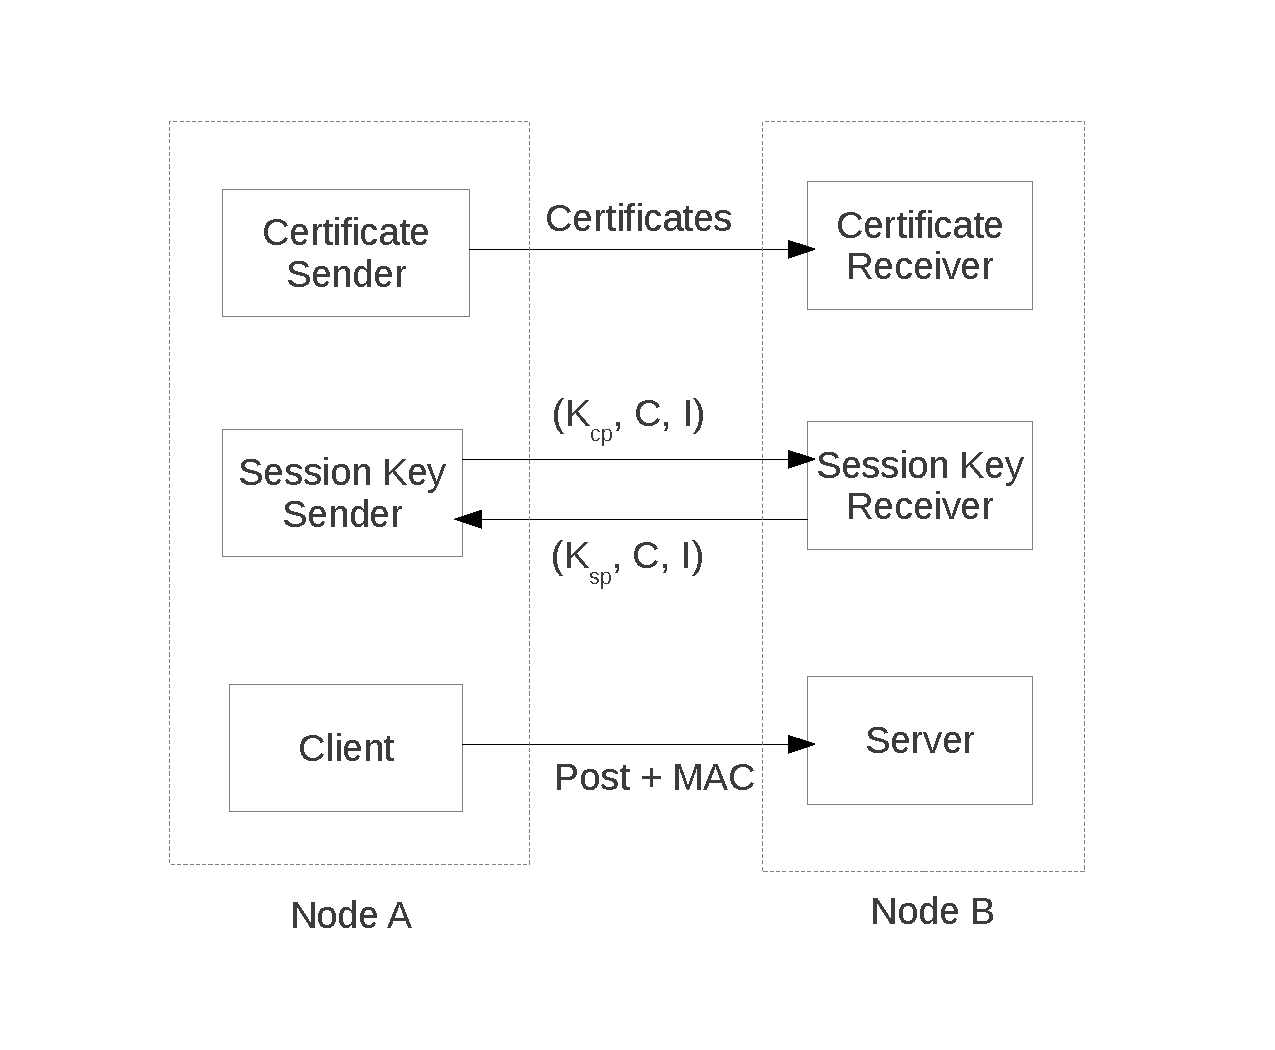
\includegraphics{Figures/SprocketRT-Protocol.pdf}}}
\stopslide

%%%%%

\startslide{Certificate Receiver}
\centerline{\scalebox{0.55}{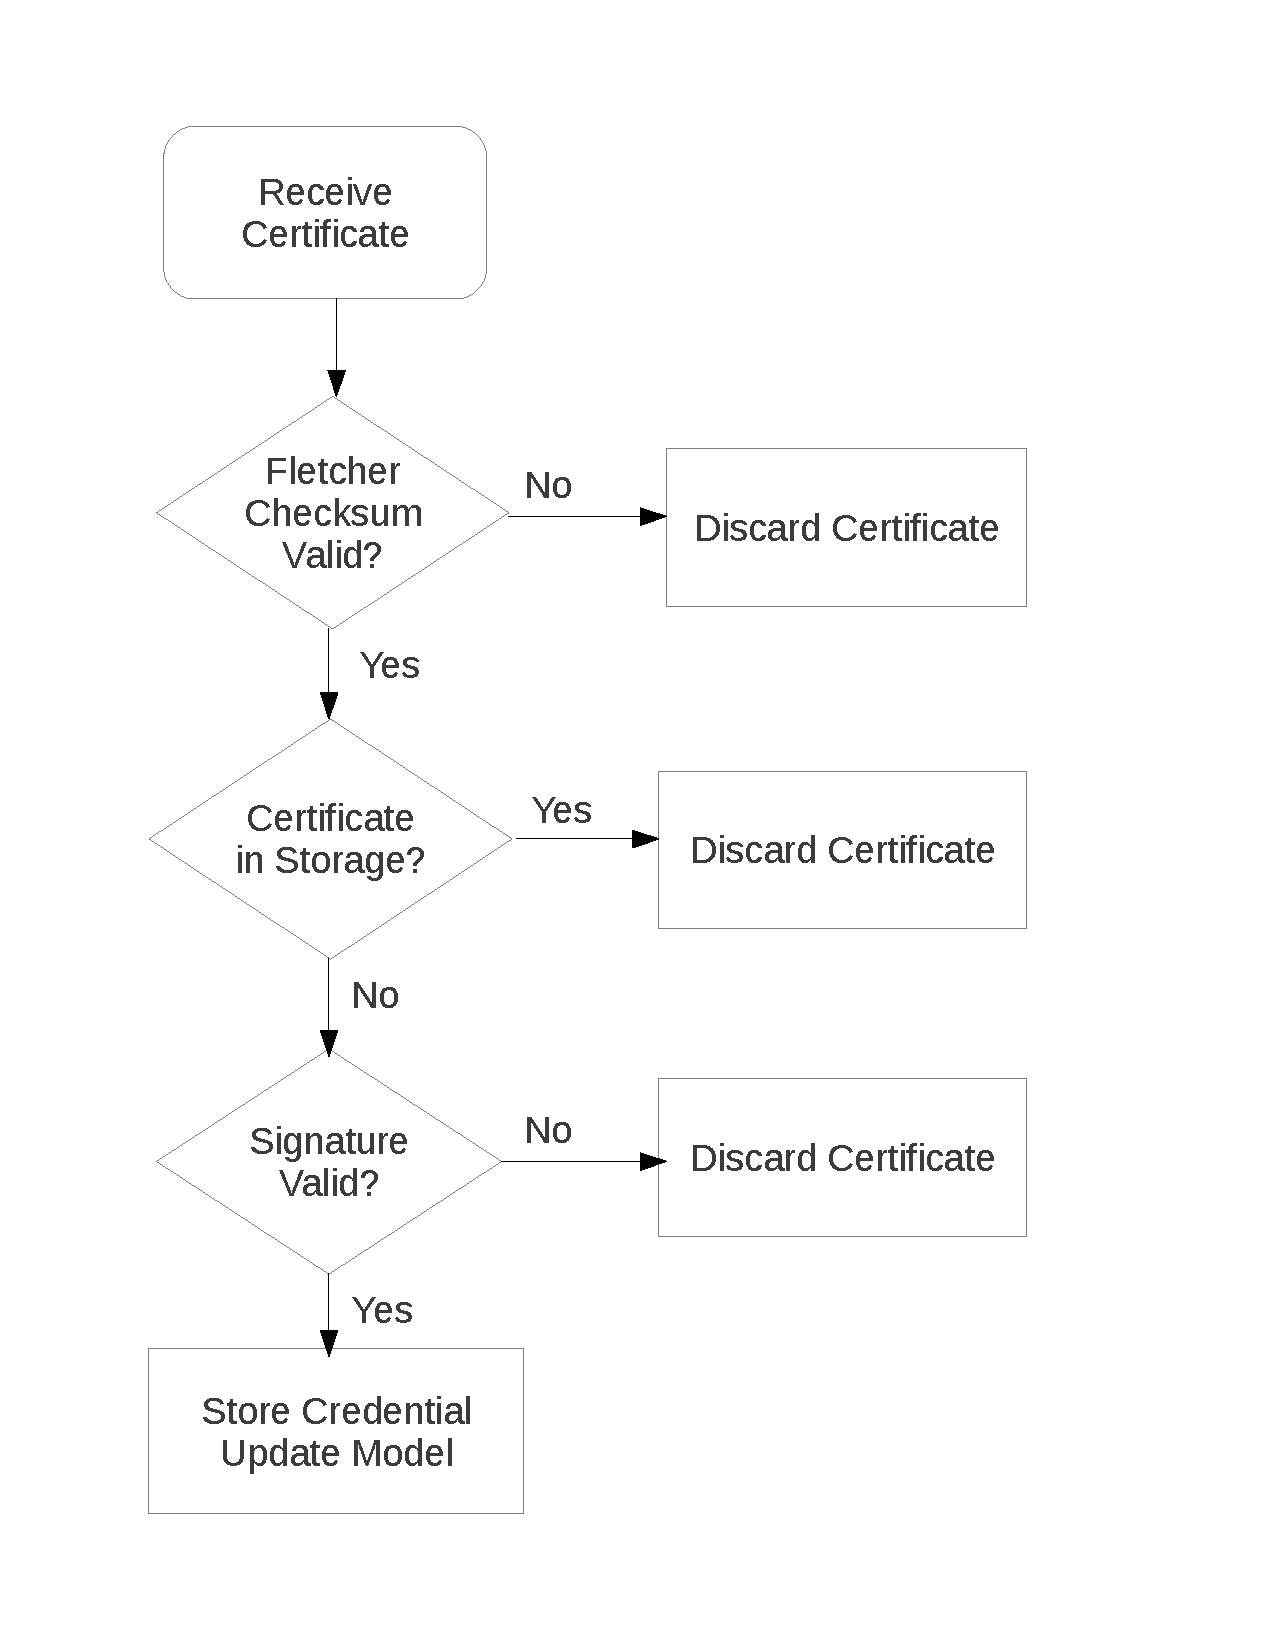
\includegraphics{Figures/Certificate-Receiver-Flowchart.pdf}}}
\stopslide

%%%%%

\startslide{Post Duty}
\centerline{\scalebox{0.70}{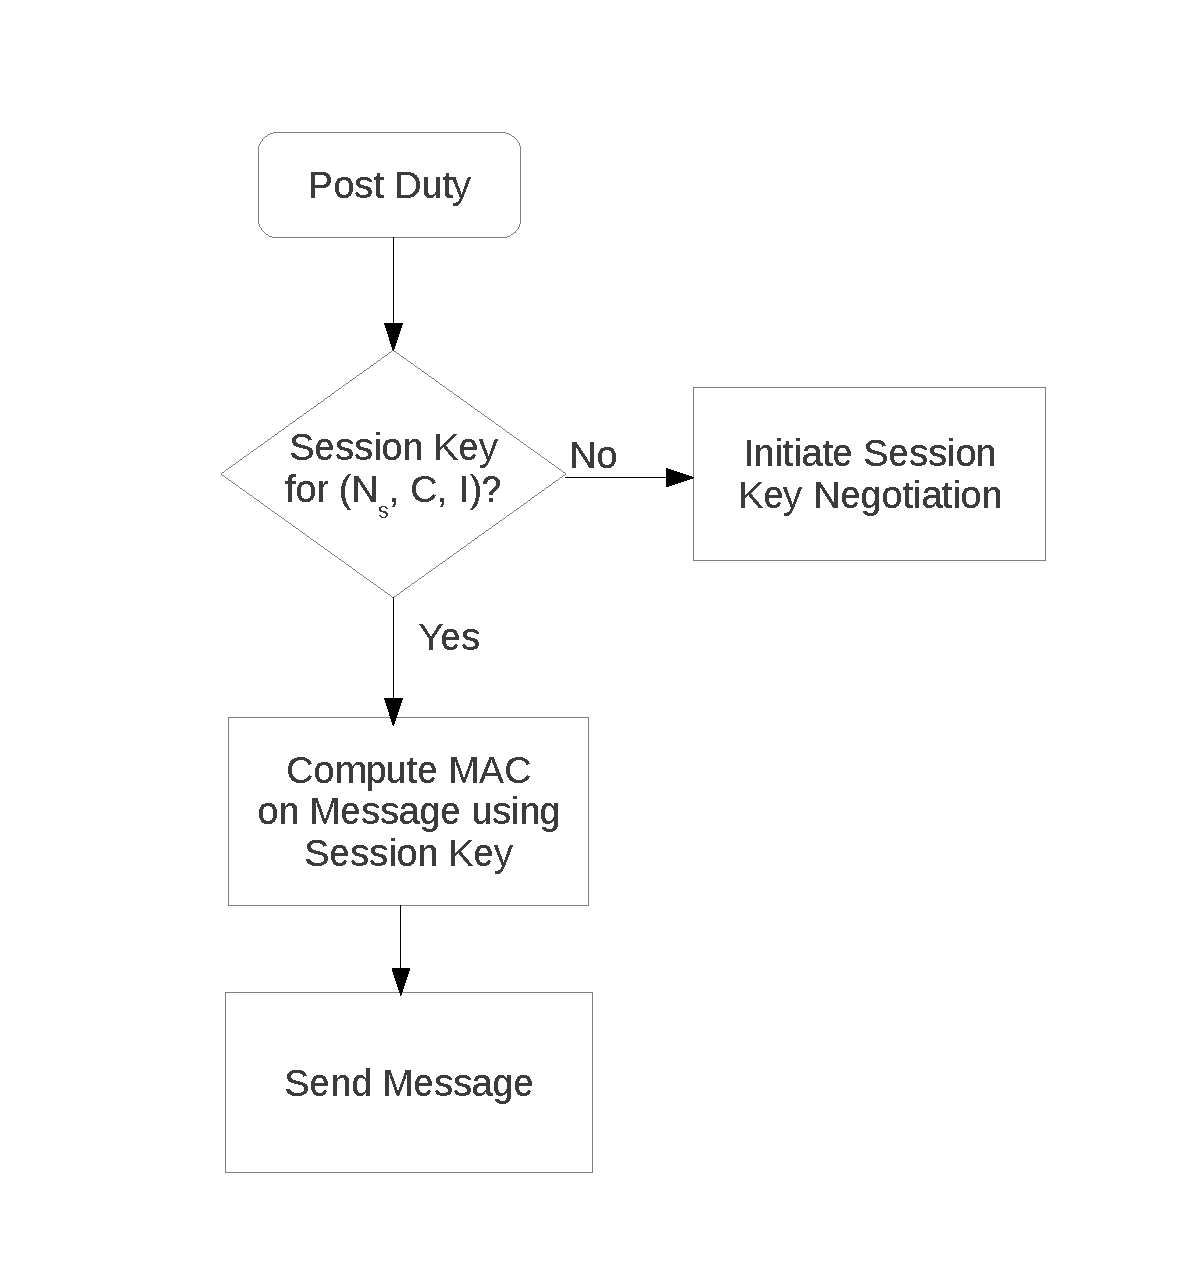
\includegraphics{Figures/Post-Duty-Flowchart.pdf}}}
\stopslide

%%%%%
%
%\startslide{Post Format}
%\centerline{\scalebox{1.0}{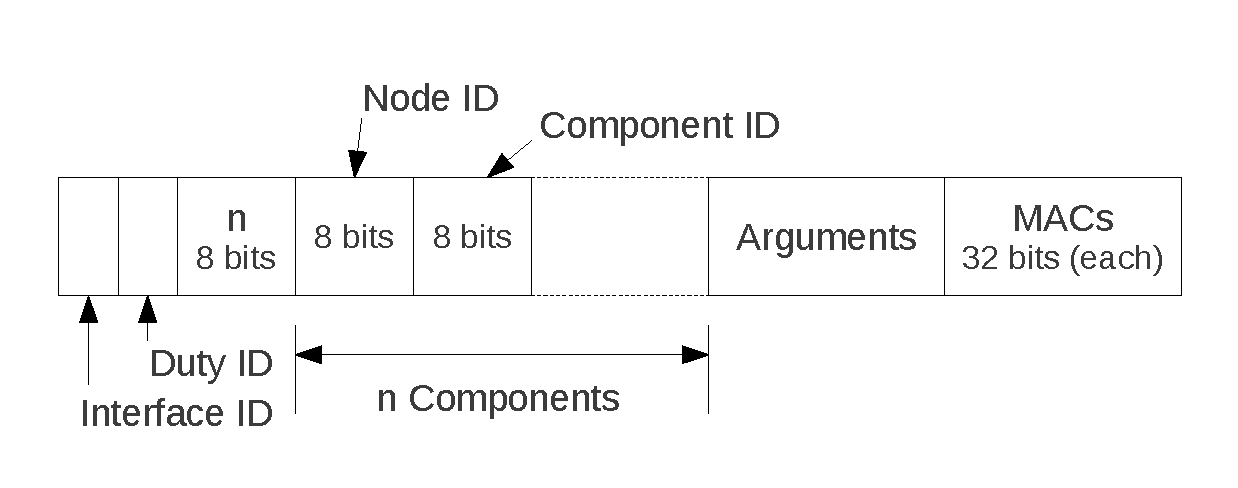
\includegraphics{Figures/Post-Format.pdf}}}
%\stopslide
%
%%%%%

\startslide{Receive Duty}
\centerline{\scalebox{0.70}{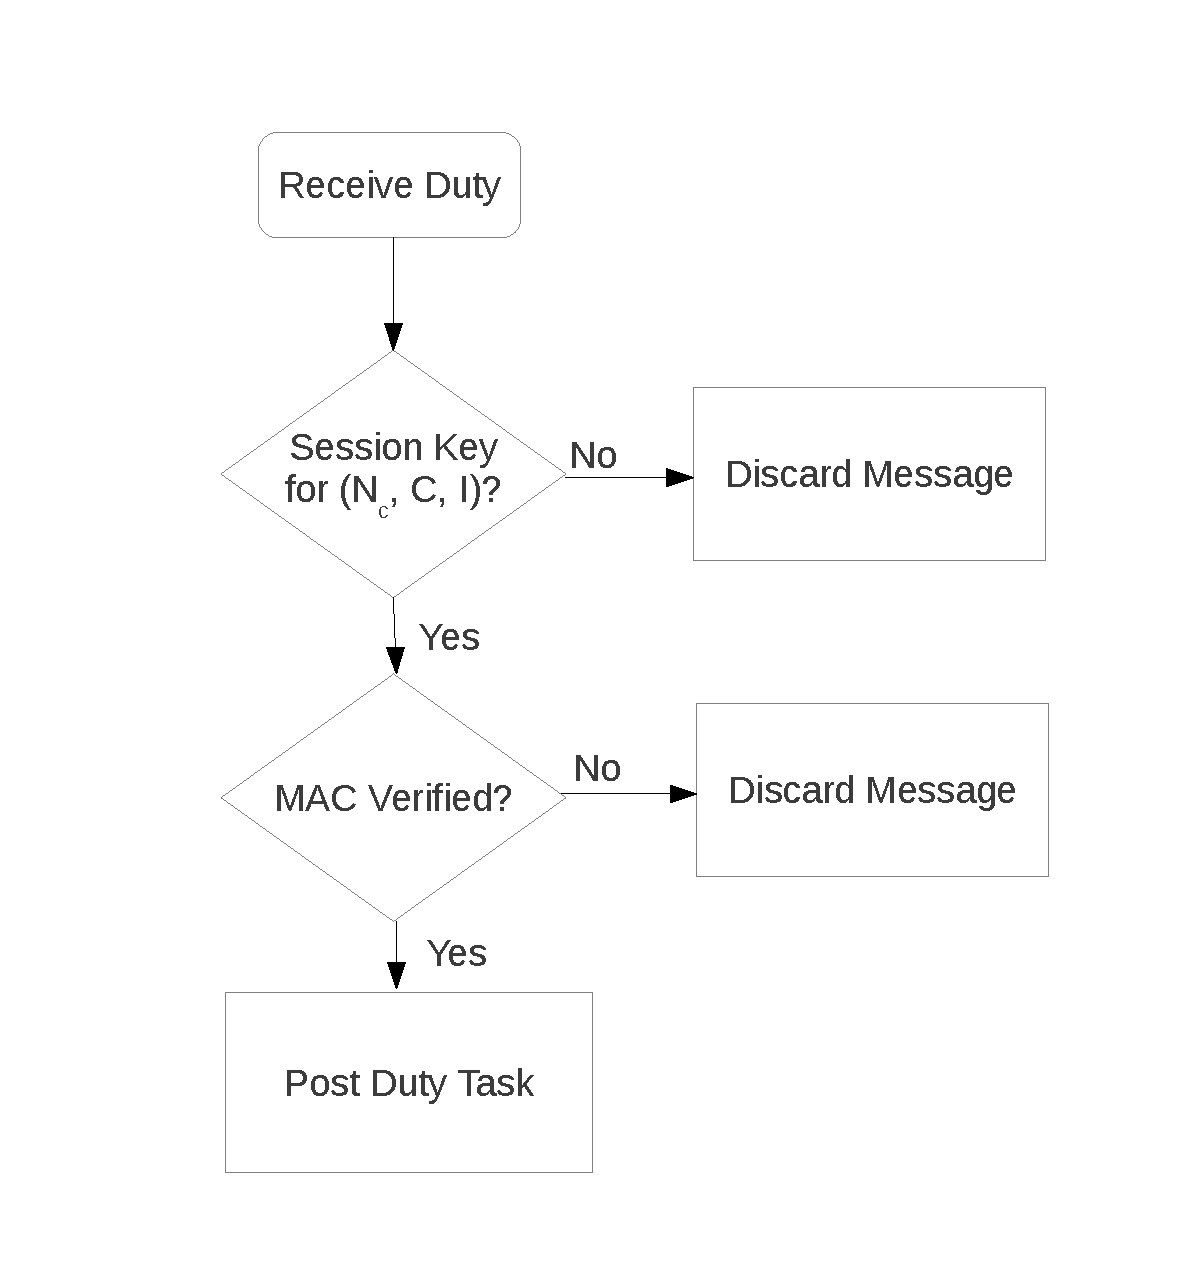
\includegraphics{Figures/Receive-Duty-Flowchart.pdf}}}
\stopslide

%%%%%
%
%\startslide{Session Key Sender}
%\centerline{\scalebox{0.85}{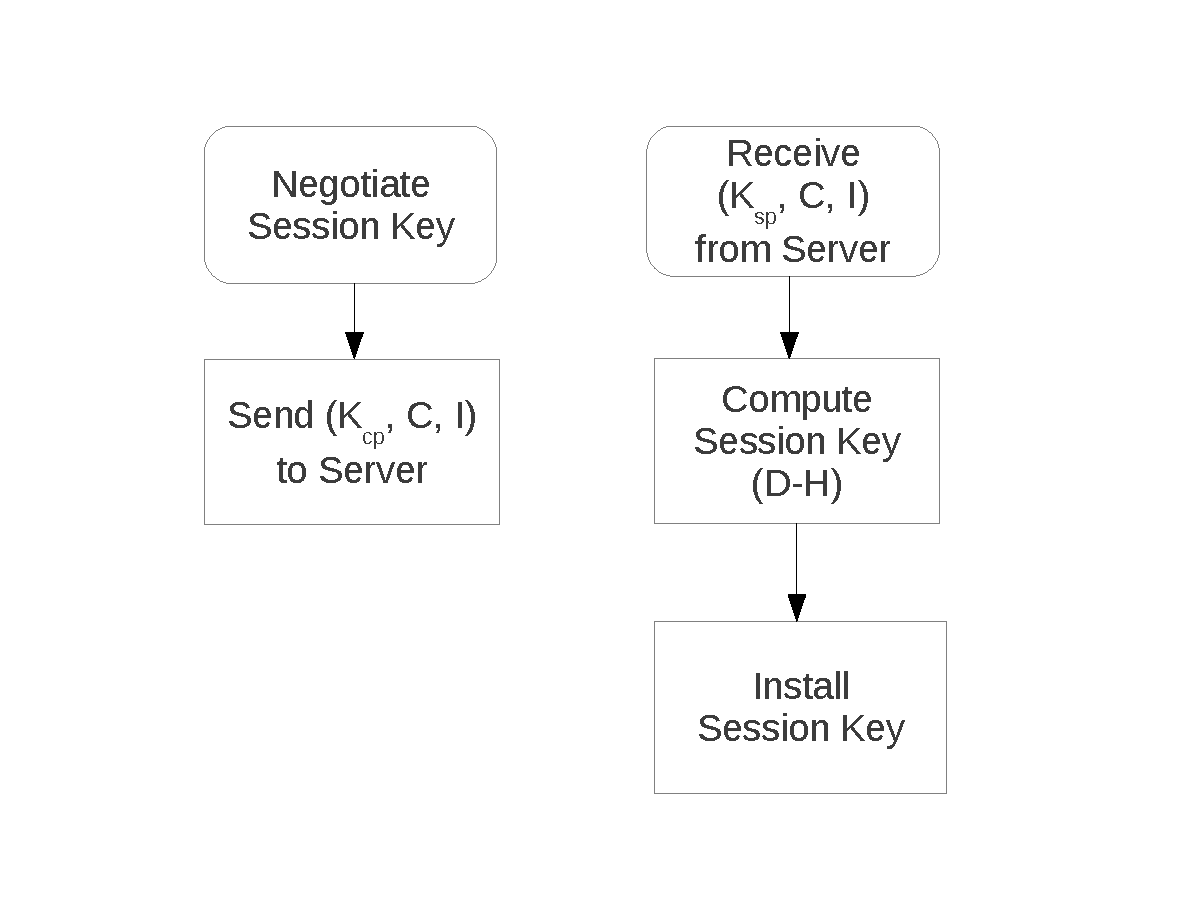
\includegraphics{Figures/SessionKey-Sender-Flowchart.pdf}}}
%\stopslide
%
%%%%%

\startslide{Session Key Receiver}
\centerline{\scalebox{0.60}{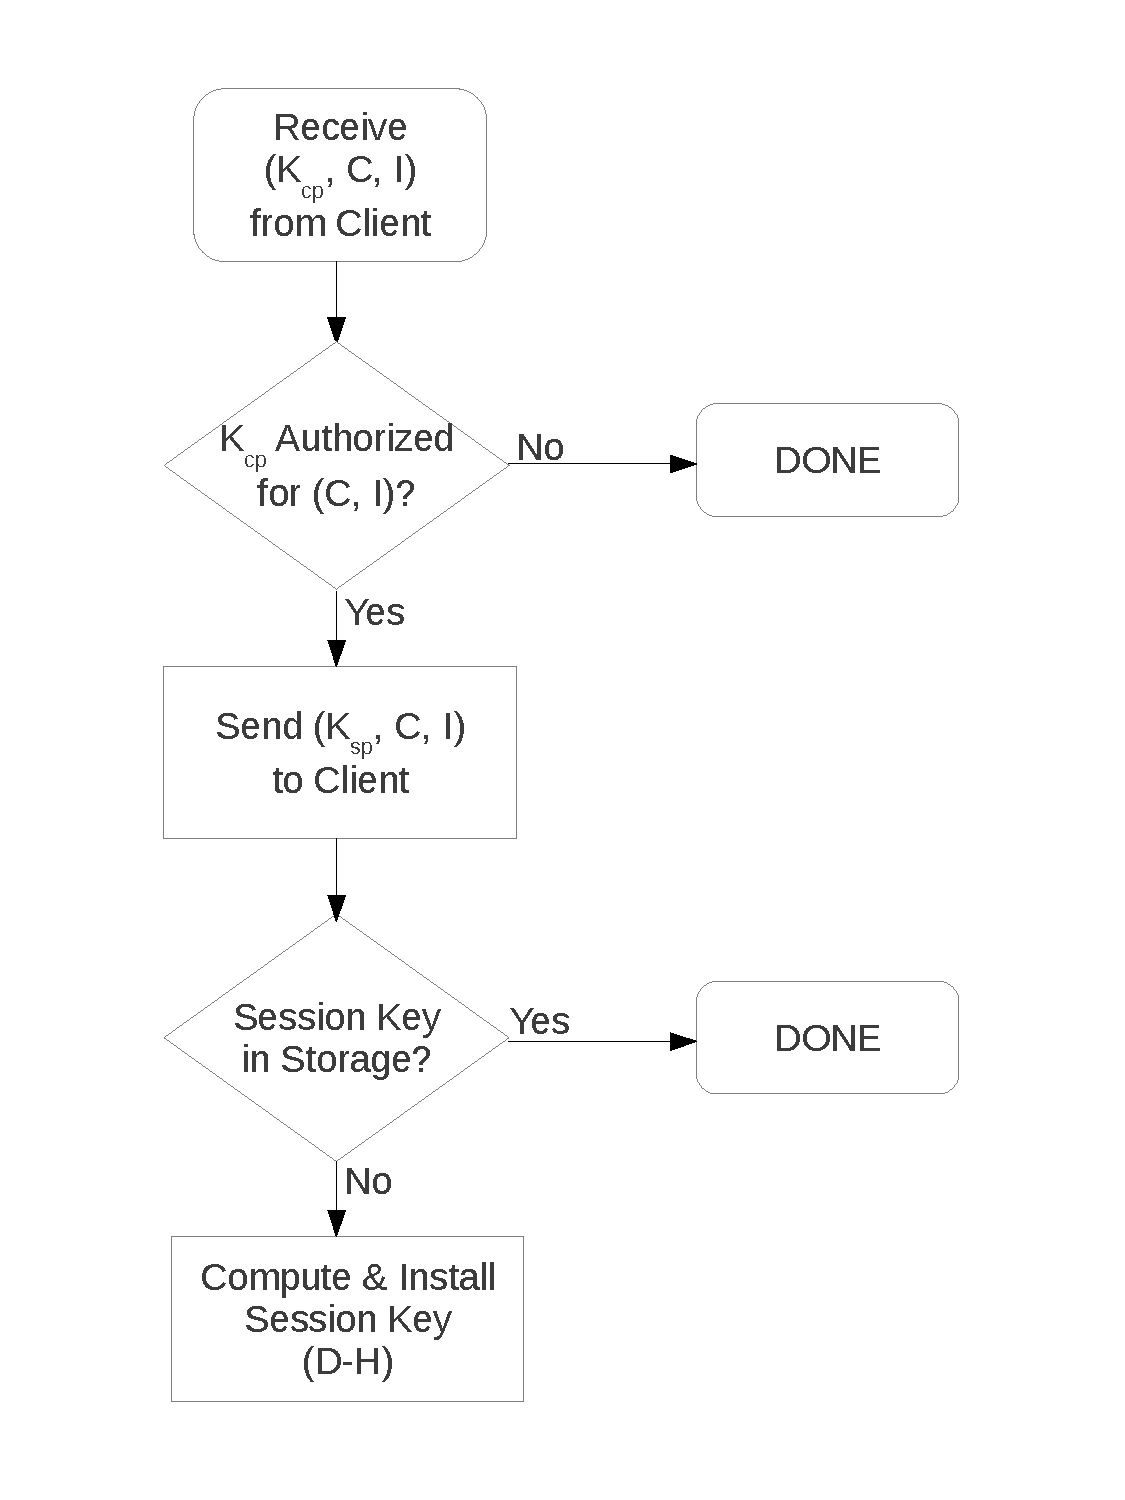
\includegraphics{Figures/SessionKey-Receiver-Flowchart.pdf}}}
\stopslide

%%%%%

\startslide{Outline}
\begin{cenumerate}
\item Introduction
\item Review of Trust Management
\item SpartanRPC/Sprocket
\item \cemph{Scalaness/nesT}
\item Evaluation
\item Conclusion
\end{cenumerate}
\stopslide

%%%%%

\startslide{Scalaness Workflow}
\centering
\scalebox{0.80}{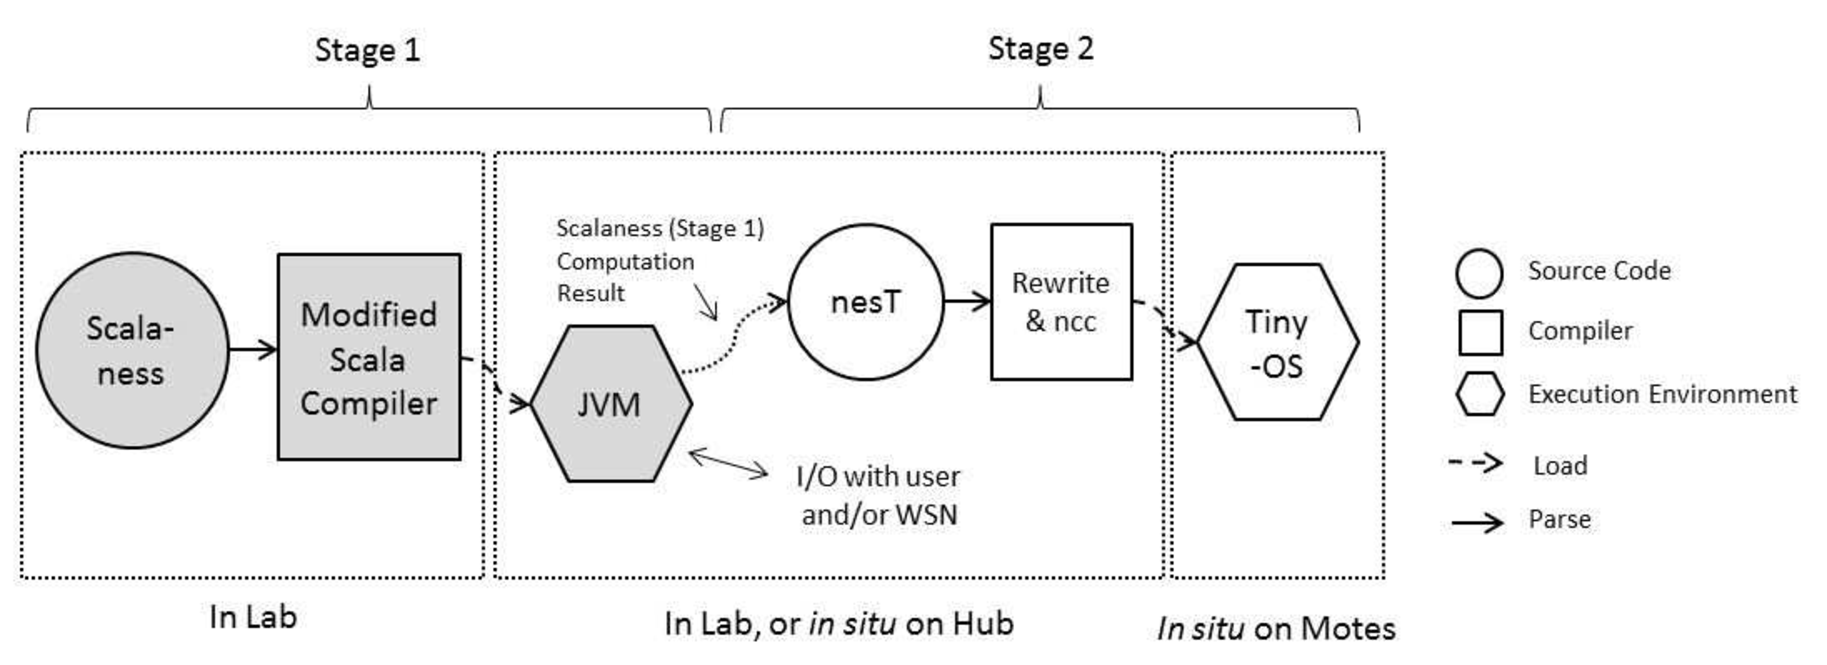
\includegraphics{Figures/scalaness.pdf}}
\begin{citemize}
\item \cemph{In the lab}: Create first stage program to specialize and compose modules of second
  stage code.
\item \cemph{In the field}: Execute first stage program to generate second stage program
  accounting for field conditions. Deploy to nodes (over the air).
\end{citemize}
\stopslide

%%%%%
%
%\startslide{The Approach}
%\begin{citemize}
%\item \cemph{Lightweight macroprogramming}: Scala at metalevel, nesC residuum, composibility at
%  the module level.
%\item Technical features: \cemph{Type specialization}, \cemph{dynamic type construction},
%  \cemph{process separation}.
%\item \cemph{Cross-stage type safety}: Type checking at Scala level ensures type safety of nesC
%  residuum.
%\item \cemph{Well-founded language design}
%\end{citemize}
%\stopslide
%
%%%%%

\startslide{Example: Introducing Some Type Abbreviations}
\lstset{basicstyle=\ttfamily, escapeinside={(*@}{@*)}}
\begin{lstlisting}[language=nesC]
(*@\tt{abbrvt\ mesgT(t) =}@*)
  { src : (*@\tt{t}@*); dest : (*@\tt{t}@*); data : uint8[] };

(*@\tt{abbrvt\ radioT =}@*)
  < at (*@$\subtype$@*) uint >
  { export error_t radio_x((*@\tt{mesgT}@*)(at)*); 
    import error_t handle_radio_r((*@\tt{mesgT}@*)(at)*); };

(*@\tt{abbrvt\ commT =}@*)
  (at (*@$\subtype$@*) uint) (*@$\circ$@*) < >
  { export error_t send((*@\tt{mesgT}@*)(at)*); 
    import error_t handle_receive((*@\tt{mesgT}@*)(at)*); };
\end{lstlisting}
\stopslide

%%%%%

\startslide{Example: nesT Modules}
\lstset{basicstyle=\ttfamily, escapeinside={(*@}{@*)}}
\begin{lstlisting}[language=nesC]
(*@\tt{authSend =}@*)
  < at (*@$\subtype$@*) uint; sendk : uint8[] >  
  { import error_t radio_x((*@\tt{mesgT}@*)(at)*);
    export error_t send(m : (*@\tt{mesgT}@*)(at)*) 
        { radio_x(AES_sign(m, sendk)); }
  };

(*@\tt{authRecv =}@*)
  < at (*@$\subtype$@*) uint; recvk : uint8[] >  
  { import error_t handle_recv((*@\tt{mesgT}@*)(at)*);
    export error_t handle_radio_r(m : (*@\tt{mesgT}@*)(at)*) 
        { if (AES_signed(m, recvk))
              handle_recv(m); }
  };
\end{lstlisting}
\stopslide

%%%%%

\startslide{Example: Scalaness Method}
\lstset{basicstyle=\ttfamily, escapeinside={(*@}{@*)}}
\begin{lstlisting}[language=scalaness]
def authSpecialize
 (nmax   : uint16,
  radioM : radioT,
  keys   : Array[Array[uint8]]) : commT {

    typedef adt (*@$\subtype$@*) uint =
      if (nmax <= 256) uint8 else uint16;

    val sendM = (*@\jinst{authSend}{adt; keys(0)}@*);
    val recvM = (*@\jinst{authRecv}{adt; keys(1)}@*);
    sendM (*@$\ltimes$@*) (*@\jinst{radioM}{adt}@*) (*@$\ltimes$@*) recvM;
}
\end{lstlisting}
\stopslide

%%%%%

\startslide{Example: Generating Residual Program}
\lstset{basicstyle=\ttfamily, escapeinside={(*@}{@*)}}
\begin{lstlisting}[language=scalaness]
val appMR =
  < >
  { export handle_recv(m : (*@\tt{mesgT}@*)(uint8)*) {(*@\ldots@*)} }; 

val appM = 
  < >
  { import send((*@\tt{mesgT}@*)(uint8)*); export main() {(*@\ldots@*)} };  

 image(appM (*@$\ltimes$@*)
         authSpecialize(nmax, radioM, keys) (*@$\ltimes$@*)
           appMR);
\end{lstlisting}
\stopslide

%%%%%
%
%\startslide{\fml\ Foundations} The \fml\ language\footnote{\cref{Yu David Liu, Christian Skalka,
%    and Scott Smith. Type-Specialized Staged Programming with Process Separation. Journal of
%    Higher Order and Symbolic Computation, 24(4):341-385, 2012.}} studies the issues at a
%foundational level.
%\begin{citemize}
%\item Comprises $F_{\le}$.
%\item MetaML-like syntax and semantics, but novel features to moderate interactions between
%  separate process spaces.
%\item Restricted form of type construction (not full $\lambda_\omega$).
%\item Formal metatheory includes cross-stage type safety---residue of partial evaluation of
%  well-typed code is guaranteed to be well-typed.
%\end{citemize}
%\stopslide
%
%%%%%

\startslide{Sample Scalaness Typing}
$$
\jmodt{\Delta_1}{\margs{\Delta_2, \Gamma}\lc 
  \imports; \exportsty \rc}
$$
Module type form, where:
\begin{citemize}
\item $\Delta_2$, $\Gamma$ type parameter bounds and term parameter types.
\item $\imports$, $\exportsty$ import and export type signatures.
\item $\Delta_1$ bounds of types constructed externally to the module.
\begin{citemize}
\item Direct substitution of these types unsound due to possible contravariant use in $\imports;
  \exportsty$.
\end{citemize}
\end{citemize}
$$
\inferrule[ModInstT]
{\Gamma \vdash \tt{e} : \jmodt{\varnothing}{\margs{\vect{t} \subtype \vect{\t}_1; 
 \vect{x} : \vect{\t}_2} \lc \imports; \exportsty \rc} \\
 \Gamma \vdash \ttvec{s} : \jinst{MetaType}{\ttvec{T}_1} \\
 \Gamma \vdash \ttvec{e}_2 : \ttvec{T}_2 \\
 \vdash \codt{\ttvec{T}_1} \subtype \vect{\t}_1 \\
 \vdash \codt{\ttvec{T}_2} \subtype \vect{\t}_2
}
{\Gamma \vdash \jinst{e}{\ttvec{s}; \ttvec{e}_2} : \jmodt{\ttvec{s} \subtype
    \codt{\ttvec{T}_1}}{\margs{} \lc \imports[\ttvec{s}/\vect{t}]; \exportsty[\ttvec{s}/\vect{t}] \rc} }
$$
\stopslide

%%%%%
%
%\startslide{Implementation}
%Scalaness/nesT has been implemented
%\begin{citemize}
%\item nesT defined as restricted subset of nesC, compiled as nesC with some rewriting
%  (e.g.~array bounds checks).
%\item Scalaness defined by extension to the Scala compiler.
%\item Type checking extends Scala type checker with module types, module operation typings, nesT
%  type checking.
%\end{citemize}
%Web site with samples: \url{http://tinyurl.com/a85z8cu}
%\stopslide
%
%%%%%

\startslide{Outline}
\begin{cenumerate}
\item Introduction
\item Review of Trust Management
\item SpartanRPC/Sprocket
\item Scalaness/nesT
\item \cemph{Evaluation}
\item Conclusion
\end{cenumerate}
\stopslide

%%%%%

\startslide{Evaluation Goals}
\begin{citemize}

\item SpartanRPC
\begin{citemize}
\item Memory overhead
\item Degradation of message transfer rate
\item Transient (``warm up'') time vs. steady-state performance
\end{citemize}

\item Realistic Application
\begin{citemize}
\item Scalaness vs. SpartanRPC
\end{citemize}
\end{citemize}

{\small Test motes: MSP430, 8\,MHz, 48\,KiB ROM, 10\,KiB RAM, TinyOS 2.1}
\stopslide

%%%%%

\startslide{Sprocket: RAM Overhead}
\centering
  \begin{tabular}{|l|r|r|r|} \hline
    \textit{Storage Area} \T & \textit{\# Items} & \textit{Bytes/Item} & \textit{Total Bytes} \\
    \hline \hline

    Session Keys ($n_k$) \T & 10 & 22 & 220 \\ \hline 
    Public Keys ($n_p$)  \T & 12 & 40 & 480 \\ \hline
    Credentials ($n_c$ ) \T & 12 & 16 & 192 \\ \hline
    Model ($n_m$)        \T & 16 &  6 &  96 \\ \hline \hline
    \textbf{Total} \T & \multicolumn{3}{r|}{ \textbf{988} } \\ \hline
  \end{tabular}
\stopslide

%%%%%

\startslide{Sprocket: Memory Consumption of Minimal Programs}
\centering
  \begin{tabular}{|l|r|r|} \hline
    \textit{Test Program} \T & \textit{RAM Bytes} & \textit{ROM Bytes} \\
    \hline \hline

    Baseline Client    \T &  349 & 10982 \\ \hline 
    Baseline Server    \T &  283 & 10490 \\ \hline
    SpartanRPC Client  \T & 2222 & 23108 \\ \hline
    SpartanRPC Server  \T & 2126 & 23394 \\ \hline
    Directed Diffusion \T & 3105 & 27826 \\ \hline
  \end{tabular}
\stopslide

%%%%%

\startslide{Maximum Message Transfer Rate}
\centering
  \begin{tabular}{|l|r|r|} \hline
    \textit{Test} \T & \textit{messages/s} & \textit{\% Reduction} \\
    \hline \hline

    Baseline \T & 128 &   -- \\ \hline 
    Duties   \T & 119 &  7.0 \\ \hline
    MAC      \T &  87 & 32.0 \\ \hline
  \end{tabular}
\stopslide

%%%%%

\startslide{Sprocket: Processing Time for Transient Operations}
\centering
  \begin{tabular}{|l|r|} \hline
    \textit{Operation} \T & \textit{Time} \\ \hline \hline

    Certificate Verification     \T &  82s \\ \hline 
    Minimum Model Construction   \T & 370$\mu$s \\ \hline
    Session Key Negotiation      \T &  80s\\ \hline
  \end{tabular}
\stopslide

%%%%%

\startslide{Sprocket: Transient Time in Single Hop Directed Diffusion}
\centering
  \begin{tabular}{|l|r|r|r|} \hline
    \textit{\# neighbors} \T & \textit{1 Cert }
                             & \textit{2 Certs}
                             & \textit{3 Certs} \\ \hline \hline

    1 \T &  4m03s & 5m27s &  6m52s \\ \hline
    2 \T &  5m16s & 6m50s &  8m24s \\ \hline
    3 \T &  6m32s & 7m57s &  9m30s \\ \hline
    4 \T &  7m50s & 9m22s & 10m51s \\ \hline
  \end{tabular}
\stopslide

%%%%%

\startslide{Sprocket: Transient Time in Multi Hop Directed Diffusion}
\centering
  \begin{tabular}{|l|r|r|r|} \hline
    \textit{Run} \T & \textit{1 hop }
                    & \textit{2 hops}
                    & \textit{3 hops} \\ \hline \hline

                   1 \T &  4m05s & 7m24s & 9m10s \\ \hline
                   2 \T &  3m12s & 5m12s & 6m30s \\ \hline
                   3 \T &  3m57s & 7m37s & 9m15s \\ \hline
                   4 \T &  4m09s & 7m15s & 8m49s \\ \hline
    \textit{Average} \T &  3m51s & 6m52s & 8m23s \\ \hline
  \end{tabular}
\stopslide

%%%%%

\startslide{Snowcloud Application}
\begin{center}
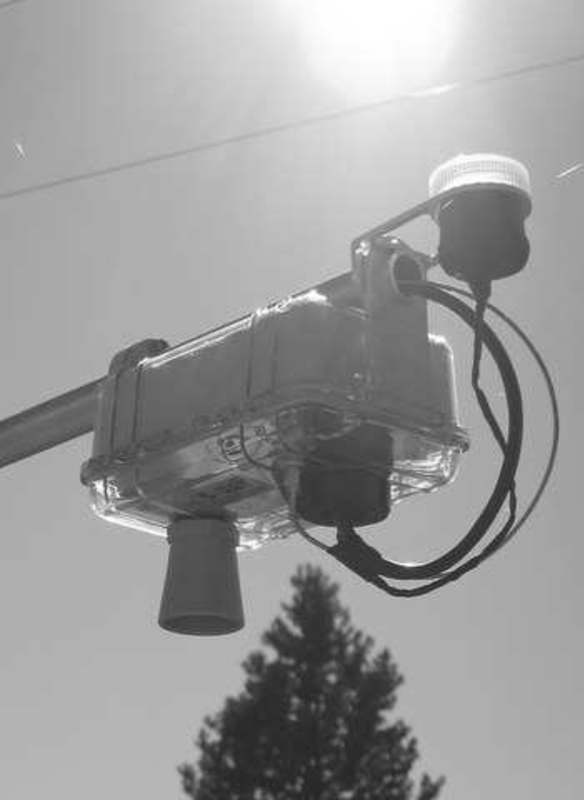
\includegraphics[scale=.50]{Figures/brainbox.pdf}
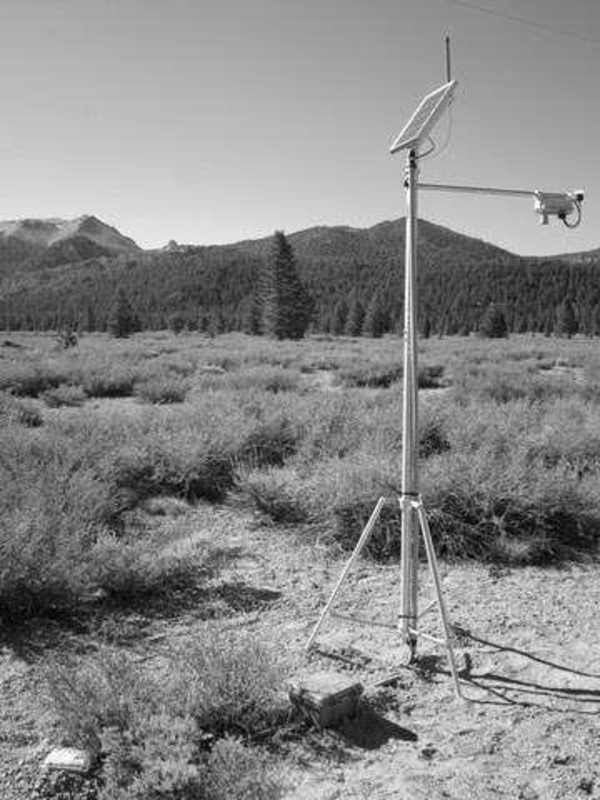
\includegraphics[scale=.50]{Figures/tower.pdf}
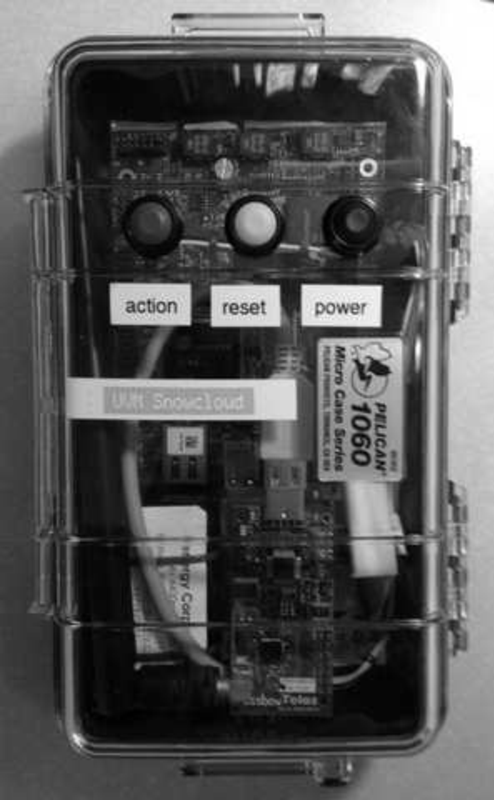
\includegraphics[scale=.50]{Figures/harvester.pdf}
\end{center}

\begin{citemize}
\item Distributed data-gathering systems for earth and agricultural sciences
\item At UVM, focus on alpine snow hydrology
\begin{citemize}
\item Deployments in California, New Hampshire, Arctic Norway
\end{citemize}
\end{citemize}
\stopslide

%%%%%

\startslide{Snowcloud Results}
\begin{center}
\begin{tabular}{|r||c|c|c|c|} \hline
              & Unsecured & Unstaged* & Staged$\dagger$ & Savings\\ \hline
Sensor ROM    &     36254 &    48616 &  36596 & 25\% \\
Sensor RAM    &      2868 &     5417 &   3038 & 44\% \\ \hline
Harvester ROM &     24316 &    35834 &  24436 & 32\% \\
Harvester RAM &      2274 &     4771 &   2402 & 50\% \\ \hline
\end{tabular}
\end{center}
\vspace{0.5in}
* Using SpartanRPC\\
$\dagger$ Using Scalaness
\stopslide

%%%%%

\startslide{Conclusion}
\begin{citemize}
\item Trust management in embedded systems is feasible.
\item SpartanRPC/Sprocket resource heavy but leaves enough for applications.
\begin{citemize}
  \item $\sim$minutes transient; $\sim$\%30 reduction in maximum message rate in
    steady-state.
\end{citemize}
\item Scalaness/nesT can dramatically improve performance.
\begin{citemize}
  \item Requires appropriate deployment scenario.
  \item Cross-stage type safety simplifies deployment.
\end{citemize}
\item Both systems could be generalized for non-sensor network applications.
\item Scalaness is far more general than SpartanRPC.
\end{citemize}
\stopslide

%%%%%

\startslide{Acknowledgments}

\centerline{I would like to acknowledge the help and advice I received from}
\centerline{\cemph{Christian Skalka, Sean Wang, and Scott Smith}}
\stopslide

%%%%%

\startslide{Questions?}
\makeatletter
\center{Peter Chapin \textless pchapin@cs.uvm.edu\textgreater}
\center{Sprocket: \cemph{https://github.com/pchapin/Sprocket}}
\center{Scalaness: \cemph{http://tinyurl.com/a85z8cu}}
\makeatother
\stopslide
